\documentclass[11pt,a4paper,oneside]{article}
% Essential
\usepackage[english]{babel}
\usepackage{fancyhdr}
\usepackage{titling}
% Optional
\usepackage{hyperref}
\usepackage{amsmath}
\usepackage{graphicx}
\usepackage{listings}
\usepackage{tikz}	
\usepackage{multicol}
\usepackage{float}
\usepackage{amsmath}
\usepackage{longtable} 
\usepackage[official]{eurosym}
\usepackage{xcolor}


\graphicspath{{figures/}}
\restylefloat{figure}
 
% Titlepage
\newcommand\maintitle{Genetic Algorithms (ATHENS course): Takehome project report}
\newcommand\teacherstitle{\large E. Sidiropoulos \\ C. Evangelides}
\title{\maintitle \\ \teacherstitle}
\date{\today}
\author{Dieter Castel}
 
% Margins
\setlength{\topmargin}{0in}
\setlength{\footskip}{0.5in}
\setlength{\textwidth}{6.5in}
\setlength{\oddsidemargin}{0in}
\setlength{\evensidemargin}{0in}
\setlength{\textheight}{8.5in}
 
% Header configuration
\pagestyle{fancy}
\fancyhead{} 
\fancyhead[L]{\maintitle}
\fancyhead[R]{\thedate}
\fancyfoot{}
\fancyfoot[L]{\theauthor}
\fancyfoot[R]{\thepage}
\renewcommand{\headrulewidth}{0.4pt}
\renewcommand{\footrulewidth}{0.4pt}

\lstdefinestyle{matlab}{
  belowcaptionskip=1\baselineskip,
  breaklines=true,
  frame=L,
  xleftmargin=\parindent,
  language=Matlab,
  showstringspaces=false,
  basicstyle=\footnotesize\ttfamily,
  keywordstyle=\bfseries\color{green!40!black},
  commentstyle=\itshape\color{purple!40!black},
  identifierstyle=\color{blue},
  stringstyle=\color{orange},
}

\begin{document}
\maketitle
\tableofcontents
%\listoffigures
%\lstlistoflistings
\newpage

\section{Introduction}
The assignment describes the problem a fire department would have if they want to select the best location for placing a fire unit.
There are 50 locations suitable and those are spaced out evenly on a grid as shown in figure \ref{fig:assig}.
The river in the center of the town has two bridges.
These bridges should be taken into account when calculating the weight each point gets according to the objective function.
The objective function models the response time to all these locations according to the distance. In the next section we will look at this function in more detail.
\begin{figure}
		\centering
		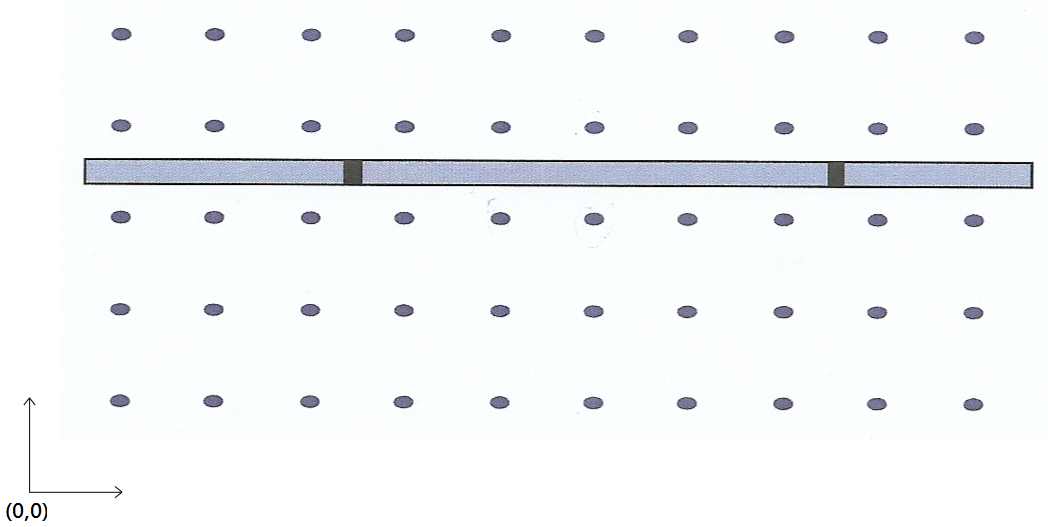
\includegraphics[scale=0.3]{assignment.png}
		\caption{Graphical representation of the town with the 50 possible locations. Each dot represents a possible building site for the fire unit. The rectangle in the center of the image is the river with the two bridges at $(3.5,3.5)$ and $(8.5,8.5)$}
		\label{fig:assig}
\end{figure}

\section{Objective function}
The objective function for this particular problem is defined as the summed distance to each of the possible building sites.
The euclidean distance is being used and the bridges are taken into account.
The euclidean distance is proffered over an other distance (e.g. hamming distance) since we have no further information about the layout of the town.
The symbolic notation of the objective function is the following:

$$f((a,b)) =  \Sigma_{x \in i, y \in j} (x - a)^2 + (y - b)^2 $$
$$\text{with } i = {1,\ldots,10}\text{ and }j ={1,\ldots,5}$$

The matlab implementation of the objective function $f$ can be found in listing \ref{l:weight} on page \pageref{l:weight}.

In figure \ref{fig:mesh} you can find a graphical representation of the objective function $f$.
The choice to represent the function in a mesh grid is intentional. 
Because creating a mesh grid isn't as calculation intensive as a more precise representation, a rough idea can quickly be formed of the function being researched.


\begin{figure}
		\centering
		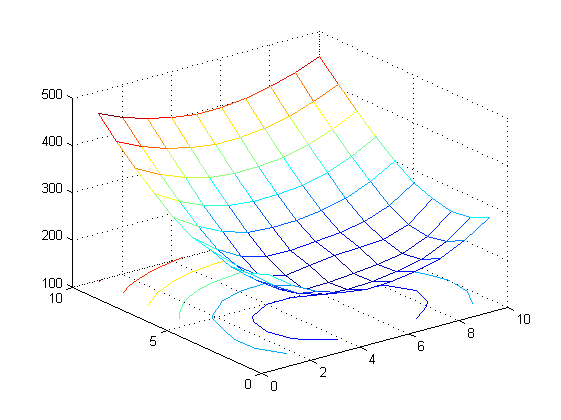
\includegraphics{mesh.png}
		\caption{A mesh visualization of the objective function. A grid of 10 on 10 is used starting in point (0,0). Under the mesh the contour plot is visible.}
		\label{fig:mesh}
\end{figure}
\section{Search space specification}
Since only a finite amount of possible locations is given the search space is clearly discrete. The (two-dimensional) points were defined in the previous section as the combination of all the elements from $i$ for the first dimension with every element of $j$ for the second dimension.

\section{Genetic Algorithm}
\subsection{code}
\lstinputlisting[style=matlab]{../ga.m}
\subsection{results}
\subsection{conclusion}
\section{Particle Swarm Optimization}
\subsection{code}
\lstinputlisting[style=matlab]{../pso.m}

\subsection{results}
\subsection{conclusion}
\section{Utility functions}
\lstinputlisting[style=matlab, caption=Matlab implementation for the objective function. The input parameter V is the vector representing the point for which the weight function $f$ is calculated., label=l:weight]{../weight.m}

\lstinputlisting[style=matlab, caption=Function that calculates the matrix holding the weights of the points generated from combining the X and Y matrices for the first and the second coordinate respectively., label=l:meshweight]{../meshweight.m}

\lstinputlisting[style=matlab, caption=Utility function that calculates the minimal euclidean distance between two given vectors taking the bridges into account., label=l:mindist]{../minDist.m}

\lstinputlisting[style=matlab, caption=Utility function that generates the possible locations for use in verious functions., label=l:loc]{../locations.m}

\end{document}
